%
% Continuous-time signals
% Commonly encountered special functions
% 
% - Dirac delta
% - Unit-step function
% - 
%
\newthought{There are two important elementary signals} which you will encounter throughout signal processing: the \emph{\index{unit impulse}{unit impulse}} $\delta(t)$ and the \emph{\index{unit step}{unit step}} function $u(t)$. Both of these functions have continuous-time and discrete-time counterparts.

\newthought{The unit impulse function $\delta(t)$} is a special distribution function\footnote{The unit impulse function is also known as the \emph{\index{Dirac delta function}{Dirac delta function}}, after physicist Paul Dirac, who used this function for modeling the distribution of electrical point-charges (e.g., electrons and protons)}, which is infinitely narrow, non-zero valued only at $t=0$. And when you integrate over this function, the result will be 1.

It is possible to define $\delta(t)$ in several different ways as a limit of functions with a well defined area and width $\sigma$. I'll use the Gaussian density function:
\begin{equation}
\delta_\sigma(t) = \frac{1}{\sqrt{2\pi \sigma^2}}e^{-\frac{t^2}{2\sigma^2}}\,\,.
\end{equation}
The Gaussian density function is shown in Figure \ref{fig:gauss_dens} for two different standard deviations $\sigma_1$ and $\sigma_2$. The smaller the value of $\sigma$, the more narrow the function is.

\begin{marginfigure}
\begin{center}
        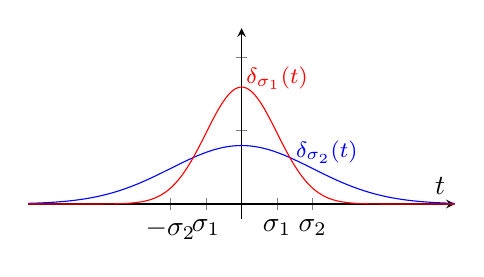
\begin{tikzpicture} \begin{axis}[width=7cm,height=4cm,ymin=-0.1,xmin=-3,ymax=1.2,xmax=3,
        yticklabels={,,}, xtick={-1,-0.5,0,0.5,1},
        xticklabels={$-\sigma_2$,$\sigma_1$,0,$\sigma_1$,$\sigma_2$},
        xlabel=$t$, axis lines = center]

%\addplot +[dirac] coordinates {(1,1.4)};
%\node at (axis cs:1.2,0.85) [below, font={\footnotesize}]{$\delta(t-t_0)$};

\node at (axis cs:1.2,0.5) [below, font={\footnotesize},color=blue]{$\delta_{\sigma_2}(t)$};
\addplot[samples=400,mark=none,color=blue]{(1/sqrt(2*3.14))*exp(-x^2/2.0)};

\node at (axis cs:0.5,1.0) [below, font={\footnotesize},color=red]{$\delta_{\sigma_1}(t)$};
\addplot[samples=400,mark=none,color=red]{(1/sqrt(2*3.14*0.25))*exp(-x^2/(2.0*0.25))};

  
\end{axis}
\end{tikzpicture}
\end{center}
\caption{A Gaussian density function becomes a unit impulse $\delta(t)$
when the width parameter approaches zero $\sigma \rightarrow 0$.}
\label{fig:gauss_dens}
\end{marginfigure}
\pgfplotsset{
    dirac/.style={
        mark=triangle*,
        mark options={scale=2},
        ycomb,
        scatter,
        visualization depends on={y/abs(y)-1 \as \sign},
        scatter/@pre marker code/.code={\scope[rotate=90*\sign,yshift=-2pt]}
    }
}
\begin{marginfigure}[0cm]
\begin{center}
        \begin{tikzpicture}
        \begin{axis}[width=7cm,height=4cm,ymin=0,xmin=-0.5,ymax=1.1,xmax=1.5,         
        yticklabels={,,},
        xtick={1},
        xticklabels={$\tau$},
        xlabel=$t$, axis lines = center]

\addplot +[dirac] coordinates {(1,1)};
\node at (axis cs:0.68,1) [below, font={\footnotesize}]{$\delta(t-\tau)$};

\end{axis}
\end{tikzpicture}
\end{center}

\caption{A unit impulse is typically depicted with a vertical arrow. A unit impulse $\delta(t-\tau)$ is centered at $t=\tau$. This is the only value of $t$ where the unit impulse is non-zero.}
\label{fig:uparrow}
\end{marginfigure}

As a result of how the function is defined, an integral over
$\delta_{\sigma}(t)$ is always unity. This is perhaps not a surprise
as this function is used in statistics as a probability density
function:
\begin{equation}
\int_{-\infty}^{\infty}\delta_\sigma(t)dt = 1 \,\,.
\end{equation}
The Dirac delta function $\delta(t)$ can be thought of as the limit when the standard deviation of this distribution approaches zero:
\begin{equation}
\lim_{\sigma\rightarrow 0}  \int_{-\infty}^{\infty} \delta_\sigma(t) dt = \int_{-\infty}^{\infty} \delta(t) dt = 1
\end{equation}
It is hopefully not difficult to convince yourself that the integral
evaluates to unity even as $\sigma \rightarrow 0$. But what does the
function $\delta(t)$ look like? First of all, it is infinitely narrow, with only one non-zero value at zero:
\begin{equation}
\delta(t) = \left\{ \begin{array}{ccc}
\infty & \mathrm{when} & t=0\\
0 &  \mathrm{when} & t \ne 0
\end{array}\right.
\end{equation}
When plotting this function, it is customary to utilize an up arrow, as shown in Figure \ref{fig:uparrow}. The figure also demonstrates how it is possible to shift the location of the peak by subtracting a constant $\tau$ from the argument of the function.

\begin{marginfigure}[0cm]
\begin{center}
        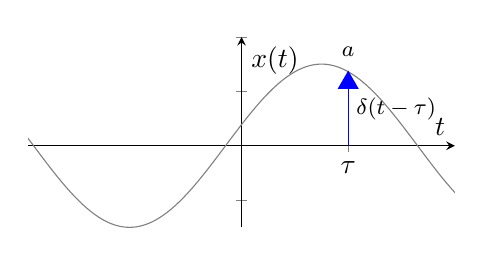
\begin{tikzpicture}
          \begin{axis}[width=7cm,height=4cm,ymin=-1.5,xmin=-2,ymax=2,xmax=2,         yticklabels={,,},
              xtick={1.0},
                      xticklabels={$\tau$},
%        xticklabels={,,},
        ylabel=$x(t)$,
    xlabel=$t$, axis lines = center]

\addplot +[dirac] coordinates {(1,1.36)};
\node at (axis cs:1.45,1.05) [below, font={\footnotesize}]{$\delta(t-\tau)$};
%\node at (axis cs:0.5,1.8) [below, font={\footnotesize}]{$x(t)$};

\node at (axis cs:1.0,2.0) [below, font={\footnotesize}]{$a$};

%\addplot[samples=400,mark=none,color=gray]{0.1*x*x*x-0.7*x*x + x + 1};
\addplot[samples=400,mark=none,color=gray]{1.5*sin(100*x+15)};
  
\end{axis}
        \end{tikzpicture}
\end{center}
\caption{The unit impulse ``selects'' the value of a continuous-time signal $x(\tau)=a$.}
\end{marginfigure}

\begin{marginfigure}
\begin{center}
        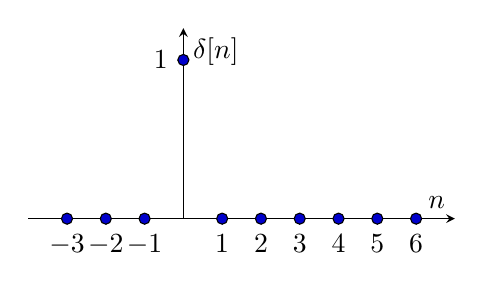
\begin{tikzpicture}
        \begin{axis}[width=7cm,height=4cm,ymin=0,xmin=-4,ymax=1.2,xmax=7,
        xtick={-3,-2,-1,0,1,2,3,4,5,6},
        ytick={0,1,2,3},
        ylabel={$\delta[n]$},
    xlabel={$n$}, axis lines = center]
   \addplot+[ycomb,color=black] plot coordinates {(-3,0) (-2,0) (-1,0) (0,1) (1,0) (2,0) (3,0) (4,0) (5,0) (6,0)};
\end{axis}
        \end{tikzpicture}
\end{center}
\caption{The discrete-time unit impulse.}
\label{fig:udensdisc}
\end{marginfigure}

The main application of the unit impulse function in signal processing is selecting or ``sampling'' a value of a signal. This is also sometimes referred to as the \emph{\index{sifting}{sifting}} property. Consider a function $x(t)$ which has the value $x(\tau) = a$. If we integrate over the function $x(t)\delta(t-\tau)$, we obtain:
\begin{equation}
\int_{-\infty}^{\infty}x(t)\delta(t-\tau) dt = x(\tau) = a\,\,.
\end{equation}
This type of integral will often appear when relating a continuous-time theory to a discrete-time theory. If you are still having a difficult time convincing yourself why the integral above results in the value it does, try thinking about it through the limit:
\begin{equation}
\lim_{\sigma\rightarrow 0}\int_{-\infty}^{\infty}x(t)\delta_{\sigma}(t-\tau) dt = x(\tau) = a\,\,.
\end{equation}
The Dirac delta function is only used in this course inside an integral, so that dealing with a singularity ($\infty$) is avoided.

\if 0
\begin{equation}
    \lim_{\sigma \rightarrow 0} \delta_{\sigma}(t) = \delta(t)\,\,,
\end{equation}
where the uniform density function $\delta_{\sigma}(t)$ is defined as:
\begin{equation}
\delta_{\sigma}(t) =\left\{ \begin{array}{cl}
\sigma^{-1}, & -\frac{1}{2}\sigma < t < \frac{1}{2}\sigma \\
0, & \mathrm{otherwise}. \end{array}
\right.\,\,.
\end{equation}
This function is identical to the probability density function of a
uniformly distributed random variable. The function
$\delta_{\sigma}(t)$ is depicted for two different values of $\sigma$
in Figure \ref{fig:udens}. It is a rectangle with width $\sigma$ on
the t-axis and an amplitude of $1/\sigma$:
\begin{marginfigure}
\begin{center}
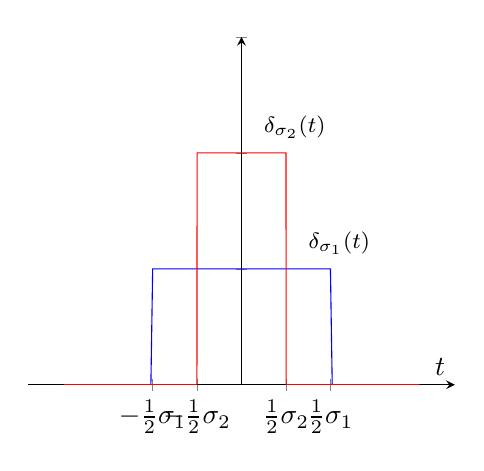
\begin{tikzpicture}
        \begin{axis}[width=7cm,height=6cm,ymin=0,xmin=-1.2,ymax=3.0,xmax=1.2,         yticklabels={,,},
        xtick={-0.5,-0.25,0.25,0.5},
        xticklabels={$-\frac{1}{2}\sigma_1$,$-\frac{1}{2}\sigma_2$,$\frac{1}{2}\sigma_2$,$\frac{1}{2}\sigma_1$},
    xlabel=$t$, axis lines = center]
\addplot[color=blue] plot coordinates {(-1,0) (-0.51,0.0) (-0.5,1.0)(0.5,1.0) (0.51,0.0) (1,0)};
\addplot[color=red] plot coordinates {(-1,0) (-0.251,0.0) (-0.25,2.0)(0.25,2.0) (0.251,0.0) (1,0)};

\node at (axis cs:0.55,1.4) [below, font={\footnotesize}]{$\delta_{\sigma_1}(t)$};

\node at (axis cs:0.3,2.4) [below, font={\footnotesize}]{$\delta_{\sigma_2}(t)$};
\end{axis}
\end{tikzpicture}
\end{center}
\caption{A rectangular pulse signal becomes a unit impulse when the width parameter $\sigma_1 \rightarrow 0$ approaches zero.}
\label{fig:udens}
\end{marginfigure}
\fi

%\newthought{The unit impulse can also be defined as an infinitely narrow Gaussian density function}:

\newthought{The discrete-time unit impulse $\delta[n]$} is defined as:
\begin{equation}
\delta[n] = \left\{\begin{array}{cl}
1 &~~~ n = 0 \\
0 &~~~ n \ne 0 \\
\end{array}
\right.\,\,.
\end{equation}
The discrete-time unit impulse signal is shown in
Figure \ref{fig:udensdisc}. In most cases, the discrete-time unit
impulse serves a similar function as its continuous-time equivalent.

%\newpage
%\subsection{Unit step}

\tikzstyle{int}=[draw, minimum size=2em]
\tikzstyle{init} = [pin edge={to-,thin,black}]
\begin{marginfigure}[-3cm]
\begin{center}

        \begin{tikzpicture}
        \begin{axis}[width=7cm,height=4cm,ymin=0,xmin=-2,ymax=1.3,xmax=2, 
                ytick={0,1},
                xtick={0},                
        yticklabels={0,1},
        xticklabels={0},
        ylabel=$u(t)$,
        xlabel=$t$,        
        axis y line=middle, axis x line=bottom]


\addplot[color=blue] plot coordinates {(-3,0) (0.00001,0) (0.0,1.0) (10,1.0) };
\addplot+[only marks,mark=o,color=blue] plot coordinates {(0,0) (0.0,1)};


%\addplot[color=red] plot coordinates {(-3,0) (0.99,0) (1.0,1.0) (10,1.0) };



%\addplot[color=red] plot coordinates {(-1,0) (-0.251,0.0) (-0.25,2.0)(0.25,2.0) (0.251,0.0) (1,0)};

%\node at (axis cs:1.0,1.0) [below, font={\footnotesize}]{$u(t-\tau)$};

\end{axis}
\end{tikzpicture}
\end{center}
\caption{The unit step function $u(t)$ shown in blue transitions from 0 to 1 at the origin.}
\end{marginfigure}


\newthought{The unit step function} can be defined as
follows\footnote{This function is also called the
  \index{Heaviside-function}{Heaviside-function}, after Oliver
  Heaviside who used this function to model signals used in
  telecommunications.}:
\begin{equation}
u(t) = \left\{\begin{array}{cl}
0 &~~~ t < 0 \\
1 &~~~ t \ge 0 \\
\end{array}
\right. \,\,.
\end{equation}
It is a step-like function, which abruptly transitions to 1 at
zero. The following figure depicts the unit step function. Notice
that there is a discontinuity at $t=0$. %There are different variants
%of the unit step function that treat this discontinuity differently.

The unit step function can be used to create a rectangular function of a
certain length. Here are two ways that this can be done:
\begin{align*}
\mathrm{rect}(t,L) &= u(t)-u(t-L)\\
&= u(t) u(L-t) \,\,.
\end{align*}
Figure \ref{fig:rect_fun} shows a plot of the rectangular
function. This type of a function appears e.g., when dealing with
ideal filters that only select spectral components that lie within a
specific band of frequencies.
\begin{marginfigure}[-5cm]
\begin{center}
        \begin{tikzpicture}
        \begin{axis}[width=7cm,height=4cm,ymin=0,xmin=-1,ymax=1.3,xmax=2, 
                ytick={0,1},
        yticklabels={0,1},
        xtick={0,1},
        xticklabels={0,$L$},
        ylabel=$u(t)-u(t-L)$,
    xlabel=$t$, 
        axis y line=middle, axis x line=bottom]

\addplot[color=blue] plot coordinates {(-3,0) (0.00001,0) (0.0,1.0) (1.0,1) (1.0,0) (10,0.0) };
%\addplot+[only marks,mark=o,color=blue] plot coordinates {(0,0) (0.0,1)};
%\addplot[color=red] plot coordinates {(-1,0) (-0.251,0.0) (-0.25,2.0)(0.25,2.0) (0.251,0.0) (1,0)};
\end{axis}
\end{tikzpicture}
\end{center}
\caption{A rectangular function that is obtained using a unit step function $u(t)-u(t-L)$.}
\label{fig:rect_fun}
\end{marginfigure}

\if 0
\newthought{It is possible to relate the unit step and the unit impulse functions}.  The unit step function can be thought of as an integral over the unit impulse over the interval $[-\infty,t]$:
\begin{equation}
u(t) = \int_{-\infty}^{t} \delta(\tau) d\tau \,\,.
\end{equation}
The above suggests that we can relate the derivative of the unit step
function to the unit impulse, which is true. 

Because the unit-step function is also a special function, which has a
discontinuity, we need to study the time-derivative by investigating
the limit of a differentiable function.  Consider the following
cumulative distribution function:
\begin{equation}
u_{\Delta}(t) = \left\{\begin{array}{cl}
0, & t < 0 \\
\frac{1}{\Delta}t, & 0 \le t < \Delta \\
1, & t \ge \Delta.
\end{array}
\right\} \,\,.
\end{equation}

\begin{marginfigure}
\begin{center}
        \begin{tikzpicture}
        \begin{axis}[width=7cm,height=6cm,ymin=0,xmin=-0.5,ymax=1.3,xmax=2, 
                     ytick={0,1},
                     yticklabels={0,1},
                     xtick={0,0.5},
                     xticklabels={0,$\sigma$},
                     axis y line=middle,
                     axis x line=bottom,
                     xlabel=$t$]

\addplot[color=blue] plot coordinates {(-3,0) (0,0.0) (0.5,1.0) (5,1.0) };
%\addplot[color=red] plot coordinates {(-1,0) (-0.251,0.0) (-0.25,2.0)(0.25,2.0) (0.251,0.0) (1,0)};

\node at (axis cs:0.2,1.0) [below, font={\footnotesize}]{$u_{\sigma}(t)$};

\end{axis}
\end{tikzpicture}
\end{center}
\caption{Imagine that the unit step function jumps from $0$ to $1$ in time $\Delta t = \sigma$, and as $\sigma \rightarrow 0$, the jump becomes a vertical line.}
\end{marginfigure}
The unit step function in this case is:
\begin{equation}
u(t) = \lim_{\sigma \rightarrow 0}  u_{\sigma}(t) \,\,.
\end{equation}
The derivative of $u_{\sigma}(t)$ is defined piecewise as:
\begin{equation}
\delta_{\sigma}(t) = \frac{d}{dt}u_{\sigma}(t) =\left\{
\begin{array}{cl}
0, & t<0\\
\frac{1}{\sigma}, & 0\le t < \sigma\\
0, & \mathrm{otherwise}
\end{array}
\right\} \,\,.
\end{equation}
At the limit $\sigma\rightarrow 0$, the derivative becomes the Dirac-delta:
\begin{equation}
\lim_{\sigma \rightarrow 0 } \frac{d}{dt}u_{\sigma}(t) = \lim_{\sigma \rightarrow 0 }\delta_{\sigma}(t) = \delta(t) \,\,. 
\end{equation}
We can thus treat $u(t)$ as a cumulative distribution function of a
random variable that only has a non-zero probability density at
$t=0$. With this definition, it is possible to relate the unit impulse
with the unit step function:
\begin{equation}
\boxed{
\delta(t) = \frac{d}{dt}u(t)
} \,\,.
\end{equation}
\fi

\newthought{The discrete-time unit step $u[n]$ function} is defined as:
\begin{equation}
u[n] = \left\{\begin{array}{cl}
0 &~~~ n < 0 \\
1 &~~~ n \ge 0 \\
\end{array}
\right.\,\,.
\end{equation}
The discrete-time unit step function is shown in Figure \ref{fig:dt_ustep}.

\begin{marginfigure}[0cm]
\begin{center}
        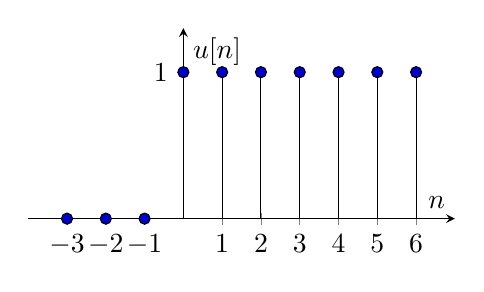
\begin{tikzpicture}
        \begin{axis}[width=7cm,height=4cm,ymin=0,xmin=-4,ymax=1.3,xmax=7,
        xtick={-3,-2,-1,0,1,2,3,4,5,6},
        ytick={0,1,2,3},
        ylabel={$u[n]$},
    xlabel={$n$}, axis lines = center]
   \addplot+[ycomb,color=black] plot coordinates {(-3,0) (-2,0) (-1,0) (0,1) (1,1) (2,1) (3,1) (4,1) (5,1) (6,1)};
\end{axis}
        \end{tikzpicture}
\end{center}
\caption{A discrete-time unit step function.}
\label{fig:dt_ustep}
\end{marginfigure}



